%!TEX encoding = UTF-8 Unicode
\documentclass{lecturenotes}

\renewcommand{\vecka}{4}
\newcommand{\veckotema}{Objekt}

%!TEX encoding = UTF-8 Unicode
\setbeamertemplate{footline}[frame number]

\newcommand{\LibVersion}{0.1.0} % latest version of introlib at https://github.com/lunduniversity/introprog-scalalib
\newcommand{\LibJar}{\texttt{introprog-\LibVersion.jar}}
\newcommand{\JDKApiUrl}{\url{https://docs.oracle.com/javase/8/docs/api/}}


\title[Föreläsningsanteckningar EDAA45, \CurrentYear]{EDAA45 Programmering, grundkurs}
\subtitle{Läsvecka \vecka: \veckotema}
\author{Björn Regnell}
\institute{Datavetenskap, LTH}
\date{Lp1-2, HT \CurrentYear}

%!TEX encoding = UTF-8 Unicode

\newcommand{\ModWeekONE}{Introduktion}
\newcommand{\ExeWeekONE}{expressions}
\newcommand{\LabWeekONE}{kojo}


\newcommand{\ModWeekTWO}{Program, kontrollstrukturer}
\newcommand{\ExeWeekTWO}{programs}
\newcommand{\LabWeekTWO}{--}


\newcommand{\ModWeekTHREE}{Funktioner, abstraktion}
\newcommand{\ExeWeekTHREE}{functions}
\newcommand{\LabWeekTHREE}{irritext}


\newcommand{\ModWeekFOUR}{Objekt, inkapsling}
\newcommand{\ExeWeekFOUR}{objects}
\newcommand{\LabWeekFOUR}{blockmole}


\newcommand{\ModWeekFIVE}{Klasser, datamodellering}
\newcommand{\ExeWeekFIVE}{classes}
\newcommand{\LabWeekFIVE}{--}


\newcommand{\ModWeekSIX}{Mönster, felhantering}
\newcommand{\ExeWeekSIX}{patterns}
\newcommand{\LabWeekSIX}{blockbattle}


\newcommand{\ModWeekSEVEN}{Sekvenser, enumerationer}
\newcommand{\ExeWeekSEVEN}{sequences}
\newcommand{\LabWeekSEVEN}{shuffle}


\newcommand{\ModWeekEIGHT}{Matriser, typparametrar}
\newcommand{\ExeWeekEIGHT}{matrices}
\newcommand{\LabWeekEIGHT}{life}


\newcommand{\ModWeekNINE}{Mängder, tabeller}
\newcommand{\ExeWeekNINE}{lookup}
\newcommand{\LabWeekNINE}{words}


\newcommand{\ModWeekTEN}{Arv, komposition}
\newcommand{\ExeWeekTEN}{inheritance}
\newcommand{\LabWeekTEN}{snake0}


\newcommand{\ModWeekELEVEN}{Kontextuella abstraktioner, api}
\newcommand{\ExeWeekELEVEN}{context}
\newcommand{\LabWeekELEVEN}{snake1}


\newcommand{\ModWeekTWELVE}{Valfri fördjupning, Projekt}
\newcommand{\ExeWeekTWELVE}{extra}
\newcommand{\LabWeekTWELVE}{Projekt0}


\newcommand{\ModWeekTHIRTEEN}{Repetition}
\newcommand{\ExeWeekTHIRTEEN}{examprep}
\newcommand{\LabWeekTHIRTEEN}{Projekt1}


\newcommand{\ModWeekFOURTEEN}{Muntligt prov}
\newcommand{\ExeWeekFOURTEEN}{Munta}
\newcommand{\LabWeekFOURTEEN}{Munta}



\begin{document}

\frame{\titlepage}
\setnextsection{\vecka}
\section[Vecka \vecka: \veckotema]{\veckotema}
\frame{\tableofcontents}

\ifkompendium\else
\begin{Slide}{Denna vecka: Objekt}
\begin{itemize}
\item Övning \texttt{objects}:
\begin{itemize}
\item deklarera singelobjekt med funktioner och tillstånd
\item använda färdiga klasser, t.ex. \code{Color} för skapa färg-objekt
\end{itemize}

\item Laboration \texttt{blockmole}
\begin{itemize}
  \item dela upp din kod i flera singelobjekt
  \item använda färdig klass i jar-fil: \code{SimpleWindow}
  \item skapa ett grafiskt spel
\end{itemize}
\end{itemize}
\end{Slide}
\fi

%!TEX encoding = UTF-8 Unicode
%!TEX root = ../lect-w04.tex

\Subsection{Objekt}


\begin{Slide}{Vad är ett objekt?}
\begin{itemize}
\item Ett objekt är en abstraktion som finns i datorns minne och
\begin{itemize}
  \item kan innehålla \Emph{data} som objektet ''håller reda på'' och
  \item kan erbjuda \Emph{operationer} som \emph{gör} något eller ger ett \emph{värde}
\end{itemize}

\pause

\item Exempel: Sköldpaddan i Kojo 
\includegraphics[width=0.08\textwidth]{../img/turtle.png}
\begin{itemize}
  \item Vilken \Emph{data} sparas av sköldpaddan?
  \pause
  \item[] position, färg på pennan, vinkel, pennans bredd, ...

  \item Vilka \Emph{operationer} kan man be sköldpaddan att utföra?

  \item[] fram, höger, vänster, ...
  \pause


\end{itemize}

\item Terminologi:
\begin{itemize}
  \item objektets data sparas i variabler som kallas \Alert{attribut}
  \item operationerna är funktioner i objektet och kallas \Alert{metoder}
  \item alla variabelvärden utgör tillsammans objektets \Alert{tillstånd}
  \item attribut, metoder (och annat i objektet) kallas \Alert{medlemmar}
\end{itemize}
\end{itemize}
\end{Slide}


\begin{Slide}{Deklarera, skapa och använda objekt}
\begin{itemize}
  \item
\end{itemize}
\end{Slide}

\begin{Slide}{Vad är ett singelobjekt?}
\begin{itemize}
\item Ett \code{object} användas ofta för att samla \Emph{medlemmar} \Eng{members} som \Alert{hör ihop} och ge dem en egen \Emph{namnrymd} \Eng{name space}.
\item Medlemmarna kan vara t.ex.:
\begin{itemize}
\item  \code{val} \item \code{var} \item \code{def}
\end{itemize}

\item Ett sådant objekt kallas även för \Emph{modul}.\footnote{
Även paket som skapas med \code{package} har en egen namnrymd och är därmed också en slags modul. Objekt kan alltså i Scala användas som ett alternativ till paket; en skillnad är att objekt kan ha tillstånd och att objekt inte skapar underkataloger vid kompilering (det finns iofs s.k. \code{package object}) \href{https://en.wikipedia.org/wiki/Modular_programming}{en.wikipedia.org/wiki/Modular\_programming}}

\end{itemize}
\end{Slide}




\begin{Slide}{Singelobjekt och metod} \SlideFontSmall
Ett Scala-\code{object} är ett s.k. \Emph{singelobjekt} \Eng{singleton object} och finns bara i \Alert{en} enda upplaga. \\ Minne för objektets variabler allokeras första gången objektet refereras. \\ En funktion som finns i ett objekt kallas en \Emph{metod} \Eng{method}.
\begin{Code}[basicstyle=\ttfamily\fontsize{9}{11}\selectfont]
object mittBankkonto {
  val kontonr: Long        = 1234567L
  var saldo: Int           = 1000
  def ärSkuldsatt: Boolean = saldo < 0
}
\end{Code}
\begin{REPLnonum}
scala> mittBankkonto.saldo -= 25000

scala> mittBankkonto.ärSkuldsatt
res0: Boolean = true
\end{REPLnonum}

(Vi ska i nästa vecka se hur man med s.k. klasser kan skapa många upplagor av samma  typ av objekt, så att vi kan ha flera olika bankkonto.)
\end{Slide}



\begin{Slide}{Vad är ett tillstånd?}
Ett objekts \Emph{tillstånd} är den samlade uppsättningen av värden av alla de variabler som finns i objektet.
\begin{Code}[basicstyle=\ttfamily\fontsize{9}{11}\selectfont]
object mittBankkonto {
  val kontonr: Long        = 1234567L
  var saldo: Int           = 1000
  def ärSkuldsatt: Boolean = saldo < 0
}
\end{Code}
\begin{tikzpicture}[font=\large\sffamily]
\matrix [matrix of nodes, row sep=0, column 2/.style={nodes={rectangle,draw,minimum width=0.8cm}}] (mat)
{
\texttt{mittBankkonto}   &  \makebox(10,10){ }\\
%\texttt{g2}   &  \makebox(16,12){ }\\
};
\node[cloud, cloud puffs=13.0, cloud ignores aspect, minimum width=2cm, minimum height=3.8cm,
 align=center, draw] (x) at (5.8cm, -1.5cm) {
 \begin{tabular}{r l}
 \texttt{kontonr} & \fbox{1234567L} \\
 \texttt{saldo} & \fbox{1000}\\
 \end{tabular}
 };
\filldraw[black] (1.7cm,0.0cm) circle (3pt) node[] (ref) {};
 \draw [arrow, line width=0.7mm] (ref) -- (x);
% \node[cloud, cloud puffs=15.7, cloud ignores aspect, %minimum width=5cm, minimum height=2cm,
% align=center, draw] (g2) at (5cm, -2cm) {Gurka-\\objekt};
% \filldraw[black] (0.4cm,-0.4cm) circle (3pt) node[] (g2ref) {};
% \draw [arrow] (g2ref) -- (g2);
\end{tikzpicture}
\end{Slide}


\begin{Slide}{Tillståndsändring}

När en variabel tilldelas ett nytt värde sker en \Emph{tillståndsändring}. Ett \Emph{förändringsbart objekt} \Eng{mutable object} har ett \Emph{förändringsbart tillstånd} \Eng{mutable state}.

\begin{REPLnonum}
scala> mittBankkonto.saldo -= 25000

scala> mittBankkonto.saldo
res1: Int = -24000
\end{REPLnonum}
\begin{tikzpicture}[font=\large\sffamily]
\matrix [matrix of nodes, row sep=0, column 2/.style={nodes={rectangle,draw,minimum width=0.8cm}}] (mat)
{
\texttt{mittBankkonto}   &  \makebox(10,10){ }\\
%\texttt{g2}   &  \makebox(16,12){ }\\
};
\node[cloud, cloud puffs=13.0, cloud ignores aspect, minimum width=2cm, minimum height=3.8cm,
 align=center, draw] (x) at (5.8cm, -1.5cm) {
 \begin{tabular}{r l}
 \texttt{kontonr} & \fbox{1234567L} \\
 \texttt{saldo} & \fbox{-24000}\\
 \end{tabular}
 };
\filldraw[black] (1.7cm,0.0cm) circle (3pt) node[] (ref) {};
 \draw [arrow, line width=0.7mm] (ref) -- (x);
% \node[cloud, cloud puffs=15.7, cloud ignores aspect, %minimum width=5cm, minimum height=2cm,
% align=center, draw] (g2) at (5cm, -2cm) {Gurka-\\objekt};
% \filldraw[black] (0.4cm,-0.4cm) circle (3pt) node[] (g2ref) {};
% \draw [arrow] (g2ref) -- (g2);
\end{tikzpicture}
\end{Slide}




\begin{Slide}{Vad rymmer sköldpaddan i Kojo i sitt tillstånd?}
\centering
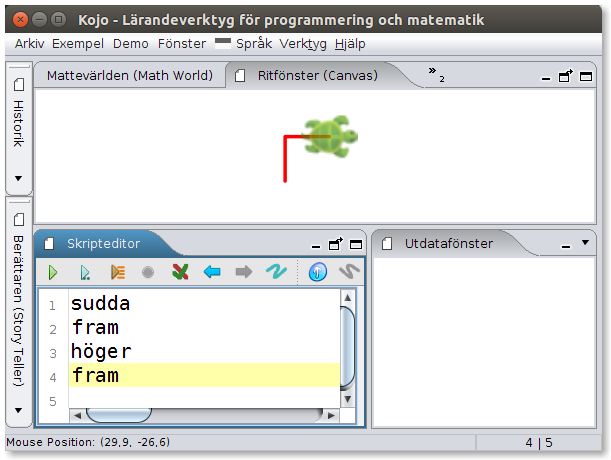
\includegraphics[width=0.7\textwidth]{../img/kojo}

\pause position, rikting, pennfärg, pennbredd, penna uppe/nere, fyllfärg
\end{Slide}




\begin{Slide}{Lata variabler och fördröjd evaluering}
Med nyckelordet \code{lazy} före \code{val} skapas en s.k. ''lat'' \Eng{lazy} variabel.
\begin{REPL}
scala> val striktVektor = Vector.fill(1000000)(math.random)
striktVektor: scala.collection.immutable.Vector[Double] =
 Vector(0.7583305221813246, 0.9016192590993339, 0.770022134260162, 0.15667718184929746, ...

scala> lazy val latVektor = Vector.fill(1000000)(math.random)
latVektor: scala.collection.immutable.Vector[Double] = <lazy>

scala> latVektor
res0: scala.collection.immutable.Vector[Double] =
  Vector(0.5391685014341797, 0.14759775960530275, 0.722606095900537, 0.9025572787055386, ...
\end{REPL}

En \code {lazy val} initialiseras \Alert{inte} vid deklarationen utan när den \Alert{refereras första gången}. Yttrycket som anges i deklarationen evalueras med s.k. \Emph{fördröjd evaluering} (även ''lat'' evaluering).
\end{Slide}

\begin{Slide}{Vad är egentligen skillnaden mellan \texttt{val}, \texttt{var}, \texttt{def} och \texttt{lazy val}?}
\begin{Code}[basicstyle=\ttfamily\fontsize{8}{11}\selectfont]
object slump {
  val förAlltidSammaReferens  = math.random
  var kanÄndrasMedTilldelning = math.random
  def evaluerasVidVarjeAnrop  = math.random
  lazy val fördröjdInit       = Vector.fill(1000000)(math.random)
}
\end{Code}
\vspace{1em}\pause
Lat evaluering är en viktig princip inom funktionsprogrammering som möjliggör effektiva, oföränderliga datastrukturer där element allokeras först när de behövs. \\
\href{https://en.wikipedia.org/wiki/Lazy_evaluation}{en.wikipedia.org/wiki/Lazy\_evaluation}
\end{Slide}





\Subsection{Funktioner är objekt}

\begin{Slide}{Programmeringsparadigm}
\href{https://en.wikipedia.org/wiki/Programming_paradigm}{en.wikipedia.org/wiki/Programming\_paradigm}:
\begin{itemize}
\item \Emph{Imperativ programmering}: programmet är uppbyggt av sekvenser av olika satser som läser och \Alert{ändrar} tillstånd
\item \Emph{Objektorienterad programmering}: en sorts imperativ programmering där programmet består av objekt som kapslar in tillstånd och erbjuder operationer som läser och \Alert{ändrar} tillstånd.
\item \Emph{Funktionsprogrammering}: programmet är uppbyggt av samverkande (matematiska) funktioner som \Alert{undviker} föränderlig data och tillståndsändringar. Oföränderliga datastrukturer skapar effektiva program i kombination med lat evaluering och rekursion.
\end{itemize}
\end{Slide}


\begin{Slide}{Funktioner är äkta objekt i Scala}
Scala visar hur man kan \Alert{förena} \Eng{unify} \\ \Emph{objekt-orientering} och \Emph{funktionsprogrammering}: \\\vspace{0.5em}

\textbf{\Large En funktion är ett objekt av funktionstyp\\ som har en \code{apply}-metod.}
\pause
\begin{REPLnonum}
scala> object öka extends (Int => Int) {
         def apply(x: Int) = x + 1
       }


scala> öka(1)
res0: Int = 2

scala> öka.   // tryck TAB
andThen   apply   compose   toString
\end{REPLnonum}
Mer om \code{extends} senare i kursen... %extends (Int => Int skrivs om till Function1[Int, Int]
\end{Slide}



\Subsection{SimpleWindow}
\begin{Slide}{Färdiga, enkla funktioner för att rita finns i klassen \texttt{cslib.window.SimpleWindow}}
På labben ska du använda \code{cslib.window.SimpleWindow}
\begin{itemize}
\item Paketet \code{cslib} innehåller paketet \code{window} som innehåller Java-klassen \code{SimpleWindow}.
%\item En \Emph{klass} är en ''mall'' för att göra \Emph{objekt}.
\item Med \code{SimpleWindow} kan man skapa ritfönster.
%\item När man skapar ett objekt från en klass använder man nyckelordet \code{new}.
\item Ladda ner \url{http://cs.lth.se/pgk/cslib} och lägg sedan jar-filen den katalog där du startar REPL med: \code{scala -cp cslib.jar}
\end{itemize}
\pause
\begin{REPLnonum}
$ scala -cp cslib.jar
scala> val w = new SimpleWindow(200,200,"hejsan")
\end{REPLnonum}
\pause Studera dokumentationen för \code{cslib.window.SimpleWindow} här: \url{http://cs.lth.se/pgk/api/}
\end{Slide}


\ifkompendium\else


\Subsection{Veckans övning och laboration}

\begin{Slide}{Övning \texttt{functions}}\SlideFontTiny
\setlength{\leftmargini}{0pt}
\begin{itemize}
%!TEX encoding = UTF-8 Unicode
%!TEX root = ../exercises.tex

\item Kunna skapa och använda funktioner med en eller flera parametrar, default-argument, och namngivna argument.
\item Kunna förklara nästlade funktionsanrop med aktiveringsposter på stacken.
\item Kunna förklara skillnaden mellan äkta och ''oäkta'' funktioner.
\item Kunna applicera en funktion på alla element i en samling.

\item Kunna använda funktioner som äkta värden.
\item Kunna skapa och använda anonyma funktioner (ä.k. lambda-funktioner).

\item Känna till att funktioner kan ha uppdelad parameterlista.
\item Känna till att det går att partiellt applicera argument på funktioner med uppdelad parameterlista för att skapa s.k. stegade funktioner (ä.k. curry-funktioner).

\item Känna till rekursion och kunna beskriva vad som kännetecknar en rekursiv funktion.
%\item Känna till att man kan loopa med rekursion och att svansrekursiva funktioner kan optimeras till while-loopar.

\item Känna till att det går att skapa egna kontrollstrukturer med hjälp av namnanrop.
\item Känna till skillnaden mellan värdeanrop och namnanrop.
\item Kunna tolka en stack trace.

\end{itemize}
\end{Slide}

\begin{Slide}{Lab \texttt{blockmole}}%\SlideFontTiny
%\setlength{\leftmargini}{0pt}
\begin{itemize}
%!TEX encoding = UTF-8 Unicode
%!TEX root = ../compendium2.tex

%\item Kunna kompilera Scalaprogram med \texttt{scalac}.
%\item Kunna köra Scalaprogram med \texttt{scala}.
%\item Kunna definiera och anropa funktioner.
%\item Kunna använda och förstå default-argument.
%\item Kunna ange argument med parameternamn.
\item Kunna skapa ett större program med din egen kod efter dina egna idéer.
\item Kunna använda en editor och terminalen för att iterativt editera, kompilera, och testa din kod.
\item Kunna använda variabler i kombination med alternativ och repetetition i flera nivåer.
\item Kunna stegvis förbättra din kod för att underlätta förändring och öka läsbarhet.
\item Kunna skapa och använda abstraktioner för att generalisera och möjliggöra återanvändning av kod.

\end{itemize}

\end{Slide}
\fi


\end{document}
